\documentclass{article}

%nty = name title year
%ynt = year name title
\usepackage[style=authoryear,sorting=nty]{biblatex}
\addbibresource{/home/uzel/dev/tex/index.bib}

\usepackage{titling}
\usepackage[margin=1in]{geometry}
\usepackage{hyperref}
\hypersetup{
    colorlinks=true,
    }

\usepackage{listings}
\usepackage{color}
\definecolor{dkgreen}{rgb}{0,0.6,0}
\definecolor{gray}{rgb}{0.5,0.5,0.5}
\definecolor{mauve}{rgb}{0.58,0,0.82}
\lstset{frame=tb,
  language=Java,
  aboveskip=3mm,
  belowskip=3mm,
  showstringspaces=false,
  columns=flexible,
  basicstyle={\small\ttfamily},
  numbers=none,
  numberstyle=\tiny\color{gray},
  keywordstyle=\color{blue},
  commentstyle=\color{dkgreen},
  stringstyle=\color{mauve},
  breaklines=true,
  breakatwhitespace=true,
  tabsize=3
}

\usepackage{graphicx}

\title{Computer Programming I notes}
\author{CIS-120A-01}
\begin{document}
\maketitle

\tableofcontents

\subsection{Readings}

\begin{itemize}
        \item \href{https://www.stevenlrichardson.com/TJ2T/}{Think Java: How to Think Like a Computer Scientist}
        \item \href{https://www.stevenlrichardson.com/IPJ/}{Introduction to Programming Using Java, Eighth Edition}
        \item \href{https://en.wikibooks.org/wiki/Java_Programming}{Java Programming}
        \item \href{https://docs.oracle.com/javase/tutorial/}{The Java™ Tutorials}
\end{itemize}

\subsection{ToDo:}

\begin{itemize}
	\item Take Syllabus Quiz
	\item Exam proctoring arrangements
	\item Locate the 4 textbooks
	\item Download Eclipse
	\item Write a Java program
\end{itemize}

\subsection{Module 0}

\subsubsection{Module readings:}
\begin{itemize}
\item \url{https://en.wikibooks.org/wiki/Java_Programming/Installation}
\item \url{https://en.wikibooks.org/wiki/Java_Programming/Compilation}
\item \url{https://en.wikibooks.org/wiki/Java_Programming/Execution}
\item \url{https://en.wikibooks.org/wiki/Java_Programming/Java_IDEs}
\end{itemize}

\subsubsection{Automatic Compulation of Dependent Classes}

In Java, if you have used any reference to any other java object, then the class for that object will be automatically compiled, if that was not compiled already. These automatic compilations are nested, and this continues until all classes are compiled that are needed to run the program. So it is usually enough to compile only the high level class, since all the dependent classes will be automatically compiled.

javac ... MainClass.java

However, you can't rely on this feature if your program is using reflection to create objects, or you are compiling for servlets or for a "jar", package. In these cases you should list these classes for explicit compilation.

javac ... MainClass.java ServletOne.java ...

\subsubsection{Imports and Packages}

In Java, programs are not compiled into executable files; they are compiled into bytecode

The bytecode gets saved on the disk with the file extension .class.

Java code needs to be compiled twice in order to be executed:

1. Java programs need to be compiled to bytecode.

2. When the bytecode is run, it needs to be converted to machine code.

\subsubsection{Packages, Subdirectories, and Resources}
head file with:

import p1.MyClass;

and,

package p1;

has to be in a directory named p1.

package org.wikibooks.egn;

has to be in a directory named en which has to be a sub-directory of wikibooks which in turn has to be a sub-directory of org resulting in org/wikibooks/en

\subsubsection{Debugging and Symbolic Information}

Debugging information is generated by the compiler together with the machine code. It is a representation of the relationship between the executable program and the original source code. This information is encoded into a pre-defined format and stored alongside the machine code. Many such formats were invented over the years for different platforms and executable files.

\subsubsection{The JIT compiler}

The Just-In-Time (JIT) compiler is the compiler that converts the byte-code to machine code. It compiles byte-code once and the compiled machine code is re-used again and again, to speed up execution. Early Java compilers compiled the byte-code to machine code each time it was used, but more modern compilers cache this machine code for reuse on the machine. Even then, java's JIT compiling was still faster than an "interpreter-language", where code is compiled from high level language, instead of from byte-code each time it was used.

The standard JIT compiler runs on demand. When a method is called repeatedly, the JIT compiler analyzes the bytecode and produces highly efficient machine code, which runs very fast. The JIT compiler is smart enough to recognize when the code has already been compiled, so as the application runs, compilation happens only as needed. As Java applications run, they tend to become faster and faster, because the JIT can perform runtime profiling and optimization to the code to meet the execution environment. Methods or code blocks which do not run often receive less optimization; those which run often (so called hotspots) receive more profiling and optimization.

\subsubsection{JSE code execution}

Stand alone application refers to a Java program where both the user interface and business modules are running on the same computer. The application may or may not use a database to persist data. The user interface could be either AWT or Swing.
The application would start with a main() method of a Class. The application stops when the main() method exits, or if an exception is thrown from the application to the JVM. Classes are loaded to memory and compiled as needed, either from the file system or from a *.jar file, by the JVM.

\subsubsection{Java 'jar' class libraries}

Utility classes, framework classes, and/or third party classes are usually packaged and distributed in Java ' *.jar' files. These 'jar' files need to be put in the CLASSPATH of the java program from which these classes are going to be used.
If a jar file is executable, it can be run from the command line:

java -jar Application.jar

\subsubsection{Client Server Applications:}

The client server applications consist of a front-end, and a back-end part, each running on a separate computer. The idea is that the business logic would be on the back-end part of the program, which would be reused by all the clients. Here the challenge is to achieve a separation between front-end user interface code, and the back-end business logic code.

The communication between the front-end and the back-end can be achieved by two ways.

1. One way is to define a data communication protocol between the two tiers. The back-end part would listen for an incoming request. Based on the protocol it interprets the request and sends back the result in data form.

2. The other way is to use Java Remote Invocation (RMI). With the use of RMI, a remote object can be created and used by the client. In this case Java objects are transmitted across the network.

\subsubsection{Web Applications:}

For applications needed by lots of client installations, the client-server model did not work. Maintaining and upgrading the hundreds or thousands of clients caused a problem. It was not practical. The solution to this problem was to create a unified, standard client, for all applications, and that is the Browser.

Having a standard client, it makes sense to create a unified, standard back-end service as well, and that is the Application Server.

Web Application is an application that is running in the Application Server, and it can be accessed and used by the Browser client.

There are three main area of interest in Web Applications, those are:
\begin{itemize}
\item The Web Browser. This is the container of rendering HTML text, and running client scripts
\item The HTTP protocol. Text data are sent back and forth between Browser and the Server
\item The Web server to serve static content, Application server to serve dynamic content and host EJBs.
\end{itemize}

\section{Module 1}

\subsection{Objectives:}

We study how a computer is built, how it works, how it performs logical operations and the nature of computing. We write our first program.
\\
\\
Our learning objectives for this module are:

\begin{enumerate}
\item Demonstrate an understanding of how a computer is built and what components it is built from
\item Describe transistors, how they are built, what they can do, and how they are used in computers
\item Demonstrate you understanding of different number bases including base 2
\item Describe two abstract models of computers
\item Define the computer science terms 'instruction' and 'computing.'
\end{enumerate}

\subsection{How a Computer Works and is Built}
\subsubsection{Transistors}
A transistor is the brain cell of the computer, made from silicon, a chemical element commonly found in sand. Transistors have revolutionized electronics since they were first invented over half a century ago by John Bardeen, Walter Brattain, and William Shockley. But what are they--and how do they work?
\\
\\
It can work either as an amplifer or a switch:
\begin{itemize}
\item When working as an amplifier, it takes a small innput current and outputs a much larger electical current. Amplification comes in handy with hearing aids.
\item When working as a switch, A small charge from one side can make a much bigger current flow through another part of. Small current switches on larger one
\item Silicon is a semiconductor, when doped with other materials and added together, makes a natural transitor.

\end{itemize}

\subsubsection{Transistors, Base Two and Storing Information}
\href{https://www.youtube.com/watch?v=USCBCmwMCDA&list=PLzdnOPI1iJNcsRwJhvksEo1tJqjIqWbN-&index=3}{How Computers Work: Binary \& Data - Video}

Input is converted into binary

\begin{figure}[h]
\centering
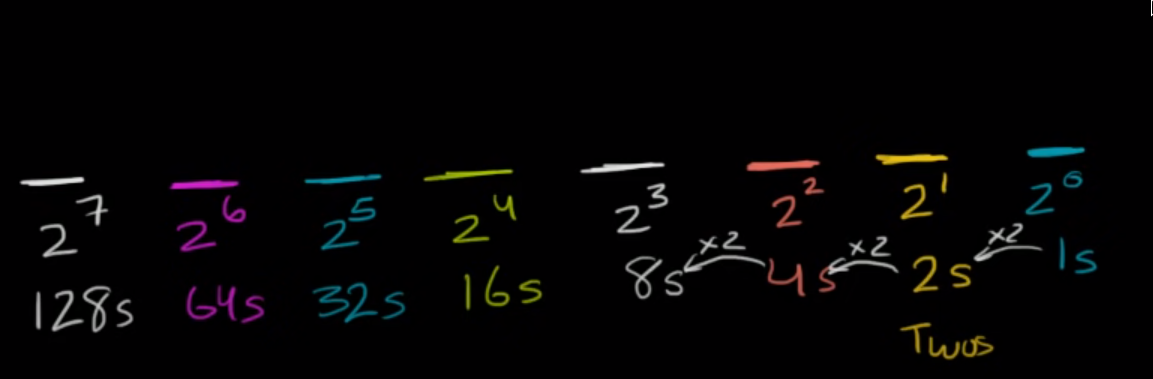
\includegraphics[width=0.7\textwidth]{~/School/fall21/CIS120A/tex/notes/images/week1/binary.png}
\caption{Binary\label{binary.png}}
\end{figure}

\begin{figure}[h]
\centering
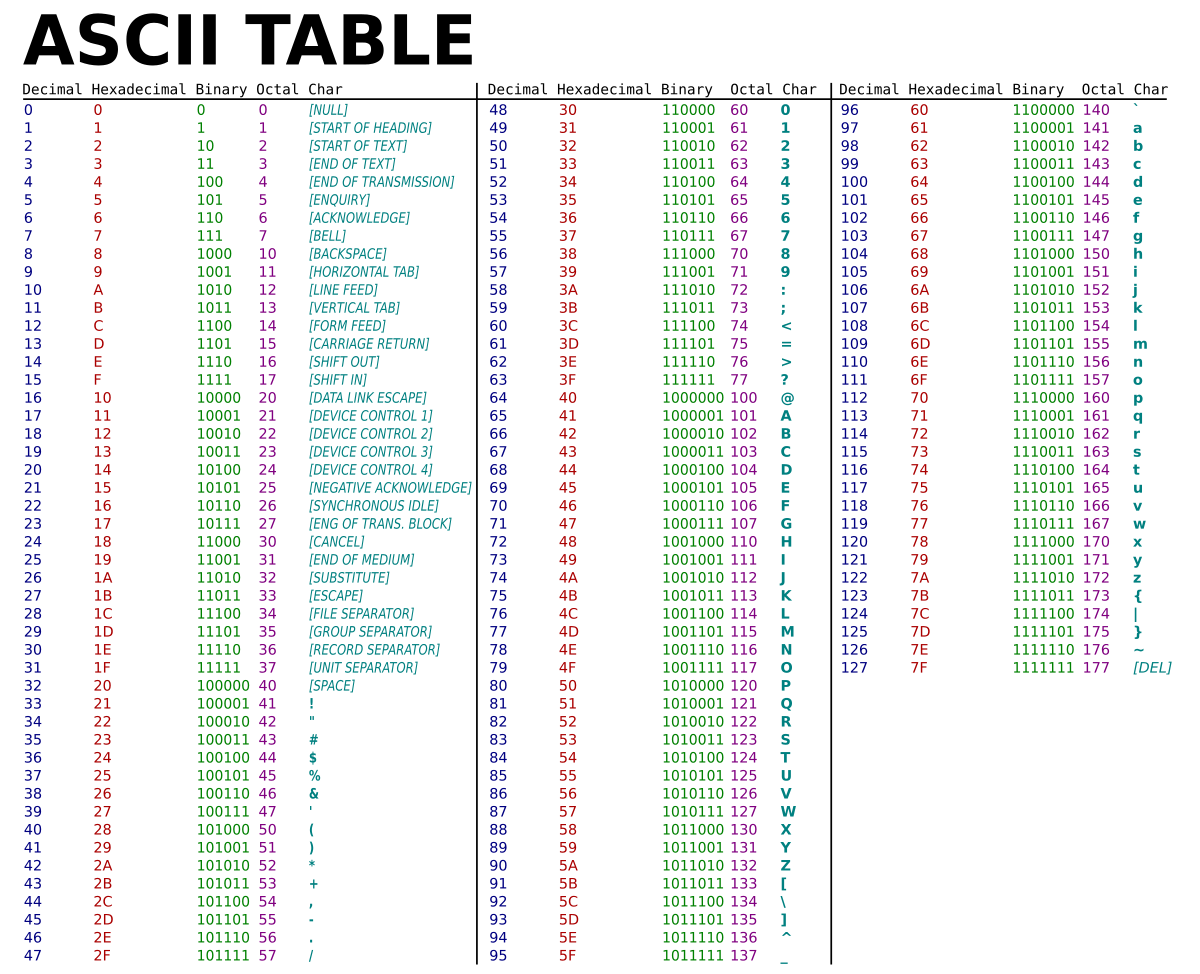
\includegraphics[width=0.7\textwidth]{~/School/fall21/CIS120A/tex/notes/images/week1/ascii.png}
\caption{Ascii\label{ascii.png}}
\end{figure}


\subsubsection{Logical Operations and Gates}

This input is processed by a logic gate after sending a command to the CPU with the instructions on what kind of binary it is sending.
\\
\\
A logic gate compares several input currents and gives a different output as a result. They allow computers to make simple decisions using a mathmatical technique called Boolean algebra. 

IF raining AND own umbrella THEN go inside.

AND = operator
\\
IF windy OR snowing THEN get coat

OR = Operator
\\
IF raining AND have umbrella OR have coat THEN ok to go outside
AND = Operator
OR = Operator
\\
\\
Using AND, OR, and other operators called NOR, XOR, NOT, and NAND, computers can add up or compare binary numbers. This is  the foundation of computer programs: the logical series of instructions that make computers do things.
\\
XOR - One or the other true, but not both
\\
\\
\href{https://en.wikipedia.org/wiki/Logic_gate}{Logic Gates - Video}
\\
\\
Normally, a junction transistor is "off" when there is no base current and switches to "on" when the base current flows. That means it takes an electric current to switch the transistor on or off. But transistors like this can be hooked up with logic gates so their output connections feed back into their inputs. The transistor then stays on even when the base current is removed. Each time a new base current flows, the transistor "flips" on or off. It remains in one of those stable states (either on or off) until another current comes along and flips it the other way. This kind of arrangement is known as a flip-flop and it turns a transistor into a simple memory device that stores a zero (when it's off) or a one (when it's on). 

\subsubsection{Computer Components}
A CPU contains an Arithmetic Logic Unit, or \textbf{ALU}, which is the part of the processor that carries out operations such as addition and subtraction. It also holds a small number of \textbf{registers}, which are small memory units capable of holding a single number. A typical CPU might have 16 or 32 "general purpose" registers, which hold data values that are immediately accessible for processing.
\\
\\
The CPU also includes special purpose registers. The most important of these is the program counter, or \textbf{PC}. The CPU uses the PC to keep track of where it is in the program it is executing. The PC simply stores the memory address of the next instruction that the CPU should execute.
\\
\\
Each Memory location holds a \textbf{byte}. 8 bits
\\
\\
You should understand this much about how computers work: Main memory holds machine language programs and data. These are encoded as binary numbers. The CPU fetches machine language instructions from memory one after another and executes them. Each instruction makes the CPU perform some very small task, such as adding two numbers or moving data to or from memory. The CPU does all this mechanically, without thinking about or understanding what it does—and therefore the program it executes must be perfect, complete in all details, and unambiguous because the CPU can do nothing but execute it exactly as written. Here is a schematic view of this first-stage understanding of the computer:

\begin{figure}[h]
\centering
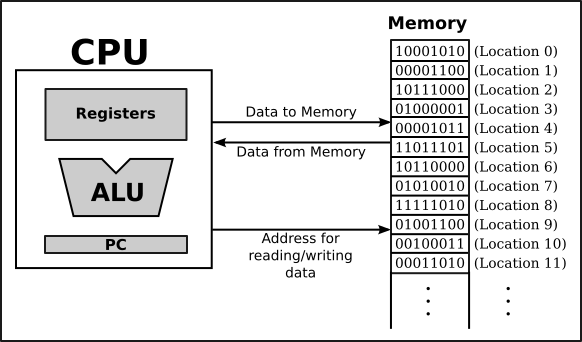
\includegraphics[width=0.5\textwidth]{~/School/fall21/CIS120A/tex/notes/images/week1/overview.png}
\caption{Overview\label{Overview.png}}
\end{figure}

There is a device driver, which consists of software that the CPU executes when it has to deal with the device. Installing a new device on a system generally has two steps: plugging the device physically into the computer, and installing the device driver software. Without the device driver, the actual physical device would be useless, since the CPU would not be able to communicate with it. (\cite{eck2018})
\\
\\
A computer system consisting of many devices is typically organized by connecting those devices to one or more \textbf{busses}. A bus is a set of wires that carry various sorts of information between the devices connected to those wires. The wires carry data, addresses, and control signals. An address directs the data to a particular device and perhaps to a particular register or location within that device. Control signals can be used, for example, by one device to alert another that data is available for it on the data bus. A fairly simple computer system might be organized like this:

\begin{figure}[h]
\centering
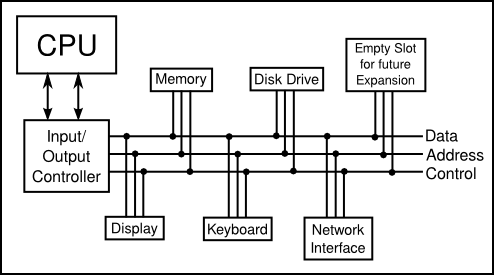
\includegraphics[width=0.5\textwidth]{~/School/fall21/CIS120A/tex/notes/images/week1/overview2.png}
\caption{Overview2\label{Overview2.png}}
\end{figure}

Now, devices such as keyboard, mouse, and network interface can produce input that needs to be processed by the CPU. How does the CPU know that the data is there? One simple idea, which turns out to be not very satisfactory, is for the CPU to keep checking for incoming data over and over. Whenever it finds data, it processes it. This method is called \textbf{polling}.
Polling is inefficient and can waste a lot of time waiting on an input signal.
\\
To avoid this inefficiency, \textbf{interrupt}s are generally used instead of polling. An interrupt is a signal sent by another device to the CPU. The CPU responds to an interrupt signal by putting aside whatever it is doing in order to respond to the interrupt. Once it has handled the interrupt, it returns to what it was doing before the interrupt occurred. For example, when you press a key on your computer keyboard, a keyboard interrupt is sent to the CPU. The CPU responds to this signal by interrupting what it is doing, reading the key that you pressed, processing it, and then returning to the task it was performing before you pressed the key.
\\
\\
That this is a purely mechanical process: A device signals an interrupt simply by turning on a wire. The CPU is built so that when that wire is turned on, the CPU saves enough information about what it is currently doing so that it can return to the same state later. This information consists of the contents of important internal registers such as the program counter. Then the CPU jumps to some predetermined memory location and begins executing the instructions stored there. Those instructions make up an interrupt handler that does the processing necessary to respond to the interrupt. (This interrupt handler is part of the device driver software for the device that signaled the interrupt.)

Interrupts make it possible for the CPU to deal efficiently with events that happen "\textbf{asynchronously}," that is, at unpredictable times.
\\
\\
Some computers can be used by several people at once. Since the CPU is so fast, it can quickly switch its attention from one user to another, devoting a fraction of a second to each user in turn. This application of \textbf{multitasking} is called \textbf{timesharing}.
\\
\\
4 Things common to all Computers
\begin{enumerate}
\item Input
\item Storage
\item Processing
\item Output
\end{enumerate}

Each of the individual tasks that the CPU is working on is called a \textbf{thread}. (Or a \textbf{process}; there are technical differences between threads and processes, but they are not important here, since it is threads that are used in Java.)

CPUs with multiple cores can execute multiple threads simultaneously.
\\
In general, a thread that is being executed will continue to run until one of several things happens:
\begin{itemize}
\item The thread might voluntarily \textbf{yield} control, to give other threads a chance to run.
\item The thread might have to wait for some asynchronous event to occur. For example, the thread might request some data from the disk drive, or it might wait for the user to press a key. While it is waiting, the thread is said to be \textbf{blocked}, and other threads, if any, have a chance to run. When the event occurs, an interrupt will "wake up" the thread so that it can continue running.
\item The thread might use up its allotted slice of time and be suspended to allow other threads to run. Most computers can "forcibly" suspend a thread in this way; computers that can do that are said to use \textbf{preemptive multitasking}. To do preemptive multitasking, a computer needs a special timer device that generates an interrupt at regular intervals, such as 100 times per second. When a timer interrupt occurs, the CPU has a chance to switch from one thread to another, whether the thread that is currently running likes it or not. All modern desktop and laptop computers, and even typical smartphones and tablets, use preemptive multitasking.
\end{itemize}

the ability to work with threads is fast becoming an essential job skill for programmers.

While programmers don't actually deal with interrupts directly, they do often find themselves writing \textbf{event handlers}, which, like interrupt handlers, are called asynchronously when specific events occur.

By the way, the software that does all the interrupt handling, handles communication with the user and with hardware devices, and controls which thread is allowed to run is called the \textbf{operating system}.

\subsubsection{Abstract Machines (i.e. Computers)}

An early pioneer in computing was Countess \href{https://en.wikipedia.org/wiki/Ada_Lovelace}{Ada Lovelace}, the daughter of the great British poet Lord Byron.  She worked with \href{https://en.wikipedia.org/wiki/Charles_Babbage}{Charles Babbage} and his \href{https://en.wikipedia.org/wiki/Analytical_Engine}{analytical engine}  She is described as the world's first computer programmer after her creation and presentation of an algorithm for computing Bernoulli Numbers.  She did so in addenda to a paper she translated from French.  These addenda amounted to brilliant scholarly work, credit for which was not widely bestowed upon her at the time.  But we can admire her now.
\\
Computer Science is a very young science.  In recent history some great minds have tackled the science of computing.  Notable among these is the British mathematician \href{https://www.britannica.com/biography/Alan-Turing}{Alan Turing}.  (It was recently announced that Turing would appear on the £50 note.)
\\
Turing created an (abstract) model for a computer called a \href{https://en.wikipedia.org/wiki/Turing_machine}{Turing Machine}. \href{https://www.cl.cam.ac.uk/projects/raspberrypi/tutorials/turing-machine/one.html}{Here is another link}.  This is a model of a device that reads instructions from a tape (i.e. memory) and executes them.  His creation of the mathematical model of a computer arose in his investigation of the so-called \href{https://en.wikipedia.org/wiki/Halting_problem}{halting problem}, which asks 'if I run this program will it ever finish?'
\\
(A brilliant man.  A gay man, he was essentially persecuted in Britain which in the post-WWII era still had Victorian era anti-gay laws on the books.  He died of an apparent suicide, having broken the German 'enigma' code during World War II, estimated to have saved thousands of lives and years of warfare because the allies could decipher all the German encoded military messages that were intercepted.  In 2009, then prime minister of the UK Gordon Brown \href{https://www.telegraph.co.uk/news/politics/gordon-brown/6170112/Gordon-Brown-Im-proud-to-say-sorry-to-a-real-war-hero.html}{published an apology to Alan Turing} for his gross mistreatment and acknowledging him as a war hero.)
\\
In 1945 \href{https://en.wikipedia.org/wiki/John_von_Neumann}{John von Neumann} published a paper describing the architecture of a digital computer, which has subsequently been coined the \href{https://en.wikipedia.org/wiki/Von_Neumann_architecture}{Von Neumann Architecture}.  This is the architecture that computers adhere to to this day.
\\
Such mathematical models were created so that early Computer Scientists (who were essentially all Mathematicians) could explore the science of computers and computing even without effective computers yet existing.
\\
See figure \ref{Neumann.png} for a visual

\begin{figure}[h]
\centering
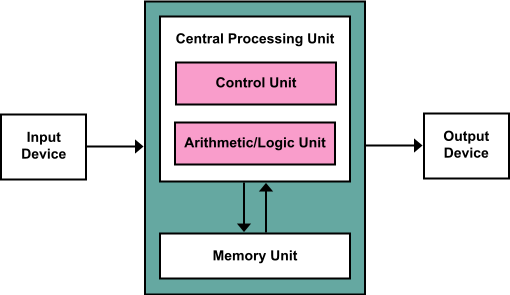
\includegraphics[width=0.7\textwidth]{~/School/fall21/CIS120A/tex/notes/images/week1/Von_Neumann_Architecture.png}
\caption{Neumann Architecture\label{Neumann.png}}
\end{figure}

\subsubsection{Instructions and Computation}
Here is an example program that creates variables named a and b and assigns the value 10 to a and the value 5 to b.  The program then swaps or interchange the values.  Run the program and see what happens:
\begin{lstlisting}
public class SwapValuesTry2 {
  public static void main(String[] args){
    int a = 10;
    int b = 5;
    //interchange (i.e. swap) the value of a and b
    int temp;  //temporary parking space for a value
    temp = a;
    a = b;
    b = temp;
    System.out.println("a is " + a + " and b is " + b);
  }
}
//a is 5 and b is 10
\end{lstlisting}

To a computer scientist, human evolution is the result of a very long computation.
It is not easy or trivial to define what is meant by a \href{https://en.wikipedia.org/wiki/Computation}{computation}, and we need much more context and experience to begin to grasp the meaning.

\subsubsection{Module 1: General Discussion}

\subsection{Getting Started with Programming \& Reading Assignment}

\subsection{What is Programming?}
\subsubsection{Methods, Classes, Programs, and Statements}
A \textbf{program} is a sequence of instructions that specifies how to perform a computation on computer hardware. 
The details look different in different languages, but a few basic instructions appear in just about every language:
\begin{itemize}
\item input: Get data from the keyboard, a file, a sensor, or some other device.
\item output: Display data on the screen, or send data to a file or other device.
\item math: Perform basic mathematical operations like addition and division.
\item decisions: Check for certain conditions and execute the appropriate code.
\item repetition: Perform some action repeatedly, usually with some variation.
\end{itemize}

Java programs are made up of \textbf{class} and \textbf{method} definitions, and methods are made up of statements. A statement is a line of code that performs a basic action.
\\
In the hello world program, this line is a print statement that displays a message on the screen:
\begin{lstlisting}
System.out.println("Hello, World!");
\end{lstlisting}

A method is a named sequence of statements. This program defines one method named main:
\begin{lstlisting}
public static void main(String[] args) 
\end{lstlisting}
The name and format of main is special: when the program runs, it starts at the first statement in main and ends when it finishes the last statement. Later, we will see programs that define more than one method.

A \textbf{class} is a collection of methods. This program defines a class named \emph{Hello}. You can give a class any name you like, but it is conventional to start with a capital letter. The name of the class has to match the name of the file it is in, so this class has to be in a file named \emph{Hello.java}.

A class can be named anything, they are usually started with a capital letter.

\subsubsection{Interpreting vs Compiling languages}

An \textbf{interpreter} reads a high-level program and executes it.
\\
\\
A \textbf{compiler} reads the entire program and translates it completely before the program starts running. In this context, the high-level program is called the source code.
\\
Java addresses the need to recompile on different machines by compiling code for a \textbf{virtual} machine. This imaginary machine’s object code is called byte code.

How does this virtual machine’s byte code get translated to the correct code for the machine we want to run our program on? The answer is an interpreter, but this time a very simple one that translates java byte code to local object code, a nearly one-for-one translation which is fast.

\subsubsection{What is Computer Science}
\href{https://google.github.io/styleguide/javaguide.html}{Google Open Source Java Styling Guide}
\\
\href{https://docs.oracle.com/javase/tutorial/}{Oracle Official Java Tutorials}
\\
\\
An \textbf{algorithm} is a sequence of steps that specifies how to solve a problem. 

\textbf{Computer science} is the science of algorithms, including their discovery and analysis.

\subsection{Excercises}

\subsubsection{One}
\begin{enumerate}
\item In computer jargon, what’s the difference between a statement and a comment?
\item What does it mean to say that a program is portable?
\item In common English, what does the word compile mean?
\item What is an executable? Why is that word used as a noun?
\end{enumerate}

Answers:
\begin{enumerate}
\item A statement is a line of code that performs a basic actions : A comment is English text that explains the code.
\item A portable program means that it can be run of different computers with few or no modifications. the compiler translates the source code into the particular machine’s object code. But if you want to move a program from machine A to machine B, you need to recompile it on machine B.
\item The process of turning source code into a machine-usable form. - A compiler reads the entire program and translates it completely before the program starts running. In this context, the high-level program is called the source code. The translated program is called the object code or the executable and is stored by the compiler for execution.
\item An executable is another name for object code that is ready to run on specific hardware.
\end{enumerate}

\subsubsection{Two}

\begin{lstlisting}
public class App {
    public static void main(String[] args) throws Exception {
        System.out.println("Hello, World!");
        System.out.println("How are you?");
        // comment
        /*
         * Multi-line Comment
         */
    }
}
\end{lstlisting}

The "Hello World!" application consists of three primary components: source code comments, the HelloWorldApp class definition, and the main method.

\subsubsection{Reading Quiz}

Question: One of the components of a computer is its CPU. What is a CPU and what role does it play in a computer?

Answer: The Central Processing Unit (CPU) is responsible for performing all of the basic calculations that it needs to with its Arithmetic Logic Unit. It is the brain of the computer, that is made up of transistors, (the brain cells)
\\
\\
Question: Explain what is meant by an "asynchronous event." Give some examples.

Answer: An asynchronous event is something that happens independent of the programs main thread.

It is something that may occur after some time and will send a signal to the CPU when it is ready to be processed, this is called an interrupt.

A thread may wait for the user to press a key, or for a file on a drive to be ready. After the CPU asks for the information, that thread is blocked, leading to other threads running. When the user presses the key or the file is ready, the thread is reactivated with an interrupt

Other examples of asyncronous events include taking input from a mic or a camera.
\\
\\
Question: What is the difference between a "compiler" and an "interpreter"?

Answer: Compilers and Interpreters both translate high-level programming languages into low-level machine language.

A compiler reads the whole high-level program and translates it entirely before running a program.

An interpreter reads and executes the high-level program line by line down the source code of the high-level program.
\\
\\
Question: Explain the difference between high-level languages and machine language.

Answer: 

High-level languages must be translated into machine code for the CPU to understand and process the information.

High-level language is portable and can run similarly on any machine, so long as it has the appropriate translator.

High-level languages are similar to traditional languages in the way they read.

Machine language is written in the binary number system. 

Machine language is not portable, meaning it is specific a certain machine.
\\
\\
Question: If you have the source code for a Java program, and you want to run that program, you will need both a compiler and an interpreter. What does the Java compiler do, and what does the Java interpreter do?

Answer: The Javac compiler compiles programs into bytecode and saves it into a .class file, which the JVM (Java Virtual Machine) is able to execute. When the JVM executes the class, the lightweight and fast Java interpreter converts java byte code into local object code (AKA Machine Language) and runs it.
\\
\\
Question: What is a subroutine (also called a method)?

Answer: A method/subroutine is a sequence of statements who has a name. 

For example,

within public static void main

main is the name of the method.
\\
\\
Question: Java is an object-oriented programming language. What is an object?

Answer: An object consists of a state and a behavior. An object stores its state into a variable. A method will affect an objects state.

\\
\\
Question: What is a variable?

Answer: A variable is the storage location for information within a computer program who is tied to a symbolic name

\\
\\
Question: Java is a "platform-independent language." What does this mean?

Answer: This means that the compiled byte code can be run seamlessly on any system that can support Java. The Java platform is always capable of interpreting the bytecode.
\\
\\
Question: What is the Java Virtual Machine?  What purpose does it serve?

Answer: The Java Virtual Machine is the platform on which compiled Java bytecode runs. This allows Java programs to be portable, meaning that they can be run on various machines with little to no modifications.

\subsection{Picobot}

room.txt

\subsubsection{Lab 0}

\subsubsection{Programming Assignment 1}

\subsection{Summary}

\section{Module 2}

\subsection{excercises}

\subsubsection{Bases and Change of Base Quiz}



\printbibliography

\end{document}

